\documentclass[parskip=full,12pt,a4paper,twoside,headings=openright]{scrreprt}
% switch to scrbook if you want roman page numbers for the front matter
% however scrbook has no 'abstract' environment!
% if your thesis is in english, use "parskip=no" instead

% binding correction (BCOR) von 1cm für Leimbindung
\KOMAoptions{BCOR=1cm}
\KOMAoptions{draft=yes}

\usepackage[utf8]{inputenc} % encoding of sources
\usepackage[T1]{fontenc}
\usepackage{studarbeit}
\usepackage{xcolor}
\usepackage{listings}
\usepackage[section]{placeins}

\title{Invasives Rust}
\author{Hermann Heinz Erich Krumrey}
\thesistype{Bachelorarbeit}
\zweitgutachter{Prof.~Dr.-Ing.~Jörg~Henkel}% for compiler stuff
\betreuer{Dipl.-Inform.~Andreas~Zwinkau}
\coverimage{coverimage/cover.png}

\newcommand{\libFIRM}{lib\textsc{Firm}}

\begin{document}

\begin{otherlanguage}{ngerman} % Titelseite ist immer auf Deutsch
\mytitlepage
\end{otherlanguage}

\begin{abstract}
\begin{center}\Huge\textbf{\textsf{Zusammenfassung}}
\end{center}
\vfill

Die Parallelisierung von Rechnern liegt immer mehr im Fokus der derzeitigen technologischen Entwicklung.
Dies erfordert die Entwicklung und Nutzung von neuen Programmierparadigmen, welche effektiv
diese neuen Architekturen ausnutzen können. Ein möglicher Ansatz ist hierbei das
invasive Computing. Dieses ermöglicht es dem Programmierer, die Ressourcennutzung
eines Programms explizit und dynamisch zu kontrollieren.

Das \textit{OctoPOS} Betriebssystem und die invasive Middleware \textit{iRTSS},
welche eine beispielhafte Implementierung für ein solches
invasives System bietet, unterstützen derzeit die Verwendung der Programmiersprachen
C, C++ als auch X10. Hiermit wird die Einführung der Programmiersprache Rust als
weitere unterstützte Sprache vorgeschlagen.

Im Rahmen dieser Arbeit wurde das \textit{octorust} Programm und die zugehörige \textit{octolib} Bibliothek
entwickelt, welche es ermöglichen, Rust auf invasiven Systemen zu verwenden. Der Einsatz von Rust
ermöglicht das speichersichere Programmieren ohne einen Garbage Collector, wobei in Folge dessen
keine Kompromisse bezüglich der Laufzeit eingegangen werden müssen. Daher bietet Rust einen
Vorteil gegenüber den bereits von \textit{OctoPOS} und \textit{iRTSS} unterstützten Sprachen.

Vorläufige Messungen haben ergeben, dass Rust in Situationen, in denen häufige Speicherallokationen und
-deallokationen vorkommen, eine über dreißig mal kürzere Laufzeit als X10 aufweisen kann, wobei bei mathematischen
Berechnungen keine eindeutige Leistungseinstufung ersichtlich ist.

\vfill

\tiny
\todo{Das Titelbild dieser Arbeit ist eine modifizierte Version des offiziellen Logos der Rust Programmiersprache. \\
Dieses ist unter der \textit{Creative Commons Attribution License (CC-BY)}
(\url{https://creativecommons.org/licenses/by/4.0/}) \\
zur Benutzung und Modifikation freigegeben.
}

\end{abstract}

\tableofcontents

\chapter{Einführung}\label{sec:intro}

Das berühmte Mooresche Gesetz besagt, dass sich die 
``Komplexität integrierter Schaltkreise mit minimalen Komponentenkosten regelmäßig verdoppelt''\cite{mooresLawWikiDe}.
Diese Beobachtung wurde im Jahre 1965 von Gordon Moore formuliert und erwies sich seither größtenteils als korrekt.
Es wird jedoch immer deutlicher, dass dieser Trend sich nicht unendlich fortsetzen kann und eventuell an physische Grenzen stößt.

Eine mögliche Lösung dieses Problems ist es, anstelle von immer schnelleren Prozessoren mehrere Prozessoren parallel zu verwenden.
Dieser Trend ist bereits zu beobachten, nahezu alle herkömmlichen Rechner oder Smartphones verfügen heutzutage über
mehrere Prozessorkerne.

Paralleles Rechnen erhöht jedoch die Komplexität des Rechnersystems als auch der darauf laufenden Software.
%TODO

Invasives Computing bietet eine mögliche  



Rust ist eine relativ neue Programmiersprache, welche verspricht 



Die Parallelisierung von Rechnern liegt immer mehr im Fokus der derzeitigen technologischen Entwicklung.
Dies erfordert die Entwicklung und Nutzung von anderen Programmierparadigmen, welche effektiv
diese neuen Architekturen ausnutzen können. Ein möglicher Ansatz ist hierbei das
invasive Computing. Dieses ermöglicht es dem Programmierer, die Ressourcennutzung
eines Programms feiner zu kontrollieren.

Das IRTSS Betriebssystem, welches eine beispielhafte Implementierung für ein solches
invasives System bietet, unterstützt derzeit die Verwendung der Programmiersprachen
C, C++ als auch X10. Hiermit wird die Einführung der Programmiersprache Rust als
weitere unterstützte Sprache vorgeschlagen. Diese Sprache hat einige wünschenswerte Merkmale, 
welche interessant für den Gebrauch im invasiven Computing sind.

Verwandte Arbeit ausm Wiki
\chapter{Grundlagen}\label{sec:basics}

Im folgenden Kapitel werden die Grundlagen der Programmiersprache Rust, der Rechnerarchitektur SPARC-V8 und des 
invasiven Computing behandelt, welche zum Verständnis dieser Arbeit beitragen.

\section{Rust}

Rust ist eine relativ neue Programmiersprache, welche wie beispielsweise C++ direkte Kontrolle über die
unterliegende Hardware bieten soll. Dies bedeutet in der Praxis, dass diese Sprache nicht von einem Garbage
Collector Gebrauch macht, wie es Sprachen wie zum Beispiel X10 tun. Im Gegensatz zu C++ bietet Rust jedoch
standardmäßig Speichersicherheit und garantieren somit dass Programme keine Speicherfehler beinhalten.
\cite{theRustLanguage}

Rust erfreut sich in der jüngsten Vergangenheit wachsende Beliebtheit bei Programmierern aller Art. So wurde
bei einer Umfrage der Webseite stackoverflow.com Rust im Jahre 2016 als beliebteste Programmiersprache bei 
Entwicklern ermittelt\cite{stackoverflowSurvey}.

Das wohl derzeit prominenteste Projekt, welches Rust verwendet, ist der Servo Web Browser Engine. Dieses Projekt
wurde von Mozilla Research initialisiert, erhält jedoch ebenfalls Beiträge von Freiwilligen
als auch von Unternehmen wie Samsung.
Diese Software soll nach und nach im Mozilla Firefox Webbrowser integriert werden und hierbei eine bessere
Leistung uns Sicherheit als vorhergehende Technologien vorweisen\cite{engineeringServo}.

\subsection{Motivation}

Eine der Kernziele der Rust Programmiersprache ist es, sichere Speicherzugriffe zu gewährleisten, ohne
für diesen Zweck einen Garbage Collector zu verwenden. Fehlerhafte Speicherzugriffe können undefiniertes
Verhalten auslösen, welches ein Sicherheitsrisiko darstellen kann, denn diese Fehler können gezielt ausgenutzt
werden, um Schadcode auszuführen.\cite{engineeringServo}\cite{undefinedBehaviour}

Außerdem soll Rust paralleles Rechnen unterstützen und so möglichst effizient moderne Hardware verwenden.
Hierfür sollen gewisse häufig auftretende Fehler in der Parallelprogrammierung gänzlich entfallen.
\cite{theRustLanguage}

Rust lehnt sich konzeptionell und syntaktisch an C-ähnliche Sprachen an, enthält jedoch auch Konzepte aus der
funktionalen Programmierung. Zusätzlich werden Sprachkonzepte und Abstraktionen geboten, welche
ansonsten zumeist in höheren Programmiersprachen geboten werden. Hierdurch soll der Einstieg für
Programmierer, die zuvor keine oder nur wenige Erfahrungen mit Systemsprachen gemacht haben, erleichtert werden.
\cite{engineeringServo}

Diese zusätzliche Sicherheiten und Nutzerfreundlichkeiten sollen jedoch keine Laufzeitkonsequenzen mit sich ziehen,
denn Rust soll in dieser Hinsicht ähnliche Ergebnisse wie andere Systemsprachen, beispielsweise C oder C++,
aufweisen. Außerdem soll Rust es vereinfachen, mehrere Programmiersprachen miteinander zu verwenden. Es soll
also möglich sein, Code aus anderen Sprachen aus einem Rust Kontext zu verwenden als auch umgekehrt.\cite{rustBook}


\subsection{Das Typsystem}

Das signifikanteste Alleinstellungsmerkmal der Programmiersprache Rust ist ihr Typsystem. Dieses ermöglicht es
erst, die versprochenen Sicherheitsgarantien ohne zusätzliche Konstrukte wie einen Garbage
Collector zu realisieren.\cite{rustBook}

\subsubsection{Ownership, Move-Semantik und Borrowing}

Das Typsystem integriert das Konzept der \textit{Ownership (engl. Besitz)} ein.
Dies ist die zentrale Besonderheit von Rusts Typsystem.
Der Grundgedanke hierhinter ist es, dass der Zugriff auf eine Speicherregion einer Variable exklusiv
zur Verfügung gestellt wird. Diese Variable wird auch\textit{Owner (engl. Besitzer)} genannt.
Zu jedem Zeitpunkt darf die Speicherregion nur einen \textit{Owner} haben.
Sobald dieser \textit{Owner} den Geltungsbereich verlässt, wird die zugehörige Speicherregion freigegeben.
Dies ist der Mechanismus, der es in Rust erlaubt, Speicher ohne manuelle Befreiung oder Nutzung eine
Garbage Collectors zu verwalten.\cite{rustBook}

Die \textit{Ownership} einer Speicherregion kann mithilfe der \textit{Move}-Semantik den Besitzer wechseln.
Die kann bei Funktionsaufrufen oder auch bei einer Zuweisung geschehen. Beispiele hierfür sind in Abbildung
\ref{code:move_semantics} zu sehen.\cite{rustBook}

\begin{lstlisting}[float,caption={Beispieldarstellung der \textit{Move}-Semantik},label=code:move_semantics]
let x = 5;    // Owner: x
let y = x;    // Owner: y, x nun ungueltig
let z = f(y)  // Ownership an f uebergeben,
              // Speicherbereich ist nun befreit,
              //   da f den Geltungsbereich verlassen hat
              // y ist ungueltig
\end{lstlisting}\cite{rustBook}

Zusätzlich zur \textit{Move}-Semantik können in Rust Referenzen zu Variablen verwendet werden. Dies wird im Kontext
von Rust häufig als \textit{borrowing (engl. ausleihen)} bezeichnet. Verwendet man eine Referenz auf eine Variable,
ist der \textit{Owner} des Speicherbereichs weiterhin die originale Variable. Es gibt zwei unterschiedliche
Typen von Referenzen, veränderliche und unveränderliche Referenzen. Standardmäßig werden in Rust unveränderliche
Referenzen verwendet. Diese erlauben es nicht, den Wert des Speicherbereichs zu verändern, sondern nur auszulesen.
Es gibt keine Limitierung bei der Anzahl unveränderlicher Referenzen eine Variable besitzen kann. Im Gegensatz
hierzu kann nur eine veränderliche Referenz auf die Variable existieren. Dies ermöglicht es, bereits zur
Compile-Zeit gewisse Wettlaufsituationen, \textit{Race Conditions}, in der Parallelprogrammierung auszuschließen. 

\subsubsection{Strukturen, Implementierungen und Traits}

Zum Erstellen von benutzerdefinierten Typen bietet Rust Strukturen (\texttt{\textsc{\textbf{struct}}}),
Implementierungen (\texttt{\textsc{\textbf{impl}}}) und Traits (\texttt{\textsc{\textbf{trait}}}).

Strukturen in Rust spezifizieren benutzerdefinierte Datentypen, welche verwandte Daten vereinen. Das Konzept
ähnelt den Strukturen in C. Anders wie in C kann man jedoch mithilfe von Implementierungen Methoden und assozierte
Funktionen für diese Strukturen definieren.
Diese Möglichkeit erlaubt es eine objektorientierte Herangehensweise in Rust zu verwenden.
Implementierungen erlauben das Definieren von Methoden, welche auf einer initiierten Struktur aufgerufen werden
und eine Referenz auf \texttt{\textsc{\textbf{self}}}, also der Struktur selbst, als Parameter entgegennehmen.
Zusätzlich können Funktionen definiert werden, welche keinen solchen Parameter entgegennehmen und somit auch mit
nicht initiierten Strukturen verwendet werden kann. Dies ähnelt statischen Methoden in objektorientierten
Sprachen.

Traits sind ein Sprachkonstrukt in Rust, welches das Verhalten von Typen abstrakt definieren können. Sie ähneln sich
hierbei Interfaces aus anderen Sprachen. 

Die \textit{}

AFFINE et LINEARE TYPEN

OWNERSHIP

TRAITS, STRUCTS, IMPLS


Eine Ausnahme hierzu bilden Type, welche das "`Copy-Trait"' oder das "`Clone-Trait"'
implementieren\cite{ownership}\cite{linearTypePain}.
So können beispielsweise Variablen vom Typ i32, welches
das "`Copy-Trait"' implementiert, beliebig oft wiederverwendet werden\cite{ownership}.
In diesem Fall existieren trotzdem nicht mehrere Zeiger auf dieselbe Speicherregion, der Speicherinhalt wird stattdessen jedes
Mal kopiert.

Ein weiteres interessantes "`Trait"' welches ein Typ in Rust implementieren kann ist das "`Drop-Trait"'\cite{dropTrait}.
Implementiert ein Typ dieses,
so kann zusätzlicher Code ausgeführt werden, sobald eine Variable von dem Typ den Geltungsbereich verlässt\cite{dropTrait}.
Dies kann hilfreich sein, um Abhängigkeiten zu behandeln, welche in einem nicht-trivialen Zusammenhang von der nun
ungültigen Variable abhängen.
Beispielsweise kann eine Netzwerkverbindung korrekt geschlossen werden sobald die dazugehörige Variable den
Geltungsbereich verlässt.

Das Ownership-System wird in der Praxis von Compiler durchgesetzt. So werden die Garantien, welche das Ownership-System
verspricht, bereits zur Compile-Zeit sichergestellt. Zusätzlich fällt die Notwendigkeit für einen Garbage Collector weg, welches
zu einer besseren Laufzeitseffizienz und Determinismus im Vergleich zu Sprachen die einen Garbage Collector verwenden beitragen.
Durch das Ownership-System entstehen keine zusätzlichen Laufzeitkosten\cite{whatIsOwnership}.

%\section{Sicherheit}

%Im folgenden wird die Sicherheit bezüglich undefiniertem Verhalten als Folge von fehlerhaften Speicherzugriffen analysiert.
%Hierbei ist vor allem der Vergleich zwischen Rust und C interessant, da einige von Rusts primären Eigenschaften die
%Risiken der C-Programmierung beseitigen sollen.

%\subsection{Division durch 0}

%Dividiert man in C einen Wert durch die Zahl 0, kann es zu undefiniertem Verhalten führen, welches auf jeden Fall unerwünscht
%ist. Versucht man dies in Rust, so bricht das Programm sofort ab, indem die "`panic\char`_fmt"'-Funktion aufgerufen wird und es
%kann nicht zu undefiniertem Verhalten kommen.

%\subsection{Pufferüberlauf}

%Ein weiterer Fall, der in C zu undefiniertem Verhalten führt, sind Pufferüberläufe. Diese geschehen, wenn man beispielsweise
%in einem Array der Größe n versucht, auf das n+1te Element zuzugreifen. Wie bereits im letzten Vergleich kann dies in 
%Rust nicht geschehen, da das Programm mit einem Aufruf der "`panic\char`_fmt"'-Funktion die Ausführung beendet.

%\subsection{Nicht Initialisierte Variablen}

%In C ist es möglich, uninitialiserte Variablen zu verwenden, dies führt allerdings ebenfalls zu undefiniertem Verhalten.
%In Rust hingegen wird dies bereits vom Compiler verhindert, da er den Gebrauch von uninitialisierten Variablen verbietet.
%Ein Rust-Programm welches also uninitialisierte Variablen verwendet kompiliert also gar nicht und kann so natürlich auch nicht
%zu undefiniertem Verhalten führen.

\subsubsection{Typsystem}

Rust verfügt über ein statisches, typsicheres Typsystem, welches sich an Typsystemen aus funktionalen Sprachen, beispielsweise Haskell, anlehnt\cite{rustWikiDe}. Dies bedeutet dass jede Variable einen eindeutigen Typ besitzt und keinen
anderen Typ annehmen kann. Rust erlaubt es zudem, per Typinferenz die explizite Angabe eines Typen bei der Variablendeklaration zu
vermeiden\cite{rustWikiDe}.

Es gibt wie in den meisten statischen Typsystemen eine Handvoll von primitiven Typen. In Rust gibt es die folgenden\cite{rustTypes}:

\begin{description}
	\item[Vorzeichenlose numerische Typen] u8, u16, u32, u64
	\item[Vorzeichenbehaftete numerische Typen im Zweier-Komplement] i8, i16, i32, i64
	\item[Platformabhängige numerische Typen] usize, isize
	\item[Textuelle Typen] char, str
\end{description}

Zudem gibt es zusätzlich noch generische Konstrukte, nämlich Tupel, Arrays, Slices, Funktionszeiger, Referenzen und Zeiger, welche
auf beliebige Typen anwendbar sind\cite{rustTypes}. Funktionen in Rust erlauben den Gebrauch für generische Typen, welches es
ermöglicht, dass eine Implementierung einer solche Funktion auf mehrere Typen anwendbar ist.

Rust borgt sich Ideen von substrukturellen Typsystemen\cite{linearTypePain}. Standardmäßig verhalten sich Variablen in Rust wie
affine Typen, welches sicherstellt, dass die Variablen höchstens ein mal verwendet werden\cite{substructuralTypesWikiEn}.
Dies wird in der Funktionsweise der "`Move"'-Semantik verdeutlicht\cite{linearTypePain}.
Es ist jedoch auch möglich, durch den Gebrauch der "`Copy"'- oder "`Clone"'-Traits Variablen
beliebig oft zu verwenden\cite{linearTypePain}.
Außerdem ist es möglich, Variablen sich wie lineare Typen verhalten zu lassen, also erzwingen dass diese Variablen mindestens
ein mal verwendet werden\cite{linearTypePain}.

Rusts Objektmodell basiert auf Strukturen, Implementierungen und Traits\cite{rustWikiEn}.
Strukturen (Schlüsselwort struct) ermöglichen die Deklaration von Feldern\cite{rustWikiEn}, 
Traits (Schlüsselwort trait) bieten Polymorphie und Vererbung
\cite{rustWikiEn} und Implementierungen (Schlüsselwort impl) erfüllen eine ähnliche Rolle wie Klassen in
anderen Programmiersprachen\cite{rustWikiEn}.

\subsubsection{Paradigmen}

Unterschiedliche Programmierparadigmen nahmen einen Einfluss auf das Sprachdesign von Rust\cite{rustWikiDe}.
Unter anderem sind Elemente der funktionalen, objektorientierten und nebenläufigen Programmierung anzutreffen\cite{rustWikiDe}.
Dies ermöglicht es unterschiedlichsten Programmierern Rust zu benutzen als auch ein hohes Abstraktionsniveau zu
bieten\cite{rustWikiDe}.

\subsubsection{Fehler- und Ausnahmebehandlung}

In der Programmiersprache Rust werden Ausnahmen behandelt, in dem die "`Option"' oder "`Result"' Aufzählung (enum) als
Rückgabeparameter einer Funktion verwendet werden. Anhand dieser kann man dann prüfen, ob eine Ausnahme beim Funktionsaufruf
aufgetreten ist. Bei unbehandelten Ausnahmen wird für den aktiven Faden (Thread) die "`panic\char`_fmt"'-Funktion aufgerufen.
Bei Fehlern beendet Rust die Ausführung des Programms. 

\subsection{Architektur/Compiler}

Der offizielle Rust Compiler heißt rustc und kann eigenständige Rust-Quelldateien kompilieren. Rust-Quelldateien haben
konventionsgemäß die Dateiendung "`.rs"'. Als Lösung zum Abhängigkeitsmanagement und der Distribution wurde das Werkzeug cargo 
entwickelt. Es ermöglicht es dem Programmierer verwendete Bibliotheken in ein Projekt einzugliedern,
indem diese in einer "`Cargo.toml"' Datei im Hauptverzeichniss
des Projekts angegeben werden. Außerdem unterstützt "`cargo"' mehrere weiter hilfreiche Funktionen zum Testen oder
Distribuieren der entwickelten Software. Kompilierte Software kann als ein sogenanntes "`Crate"' bei der
von den Rust entwickelten Platform "`crates.io"' mithilfe von cargo hochgeladen werden.

Rustc und cargo ermöglichen das Kompilieren für unterschiedliche Zielarchitekturen mithilfe der "`-{}-target"'-Option.

Um den Gebrauch von unterschiedlichen rustc und cargo Versionen zu vereinfachen, wurde das Werkzeug rustup entwickelt. Dieses
Hilfsprogramm ermöglicht es unterschiedliche Varianten des Rust-Compilers zu installieren und bei Belieben zu wechseln.
Außerdem erleichtert es die Kompilierung für anderer Zielarchitekturen, indem es für unterstützte Architekturen eine
vorkompilierte Standardbibliothek herunterladen kann.

Als Compiler-Backend wird LLVM verwendet. Durch diese wird Rust vor der Übersetzung zu Maschinenbefehlen in die Zwischensprache
LLVM-IR übersetzt. Dadurch ist es möglich, Rust-Code auf allen von LLVM unterstützen Rechnerarchitekturen laufen zu lassen.


\section{SPARC und SPARC-V8}

SPARC (\textbf{S}calable \textbf{P}rocessor \textbf{ARC}hitecture) ist eine Rechnerarchitektur, welche auf das
RISC (Reduced Instruction Set Computing) Konzept aufbaut. Eines der Ziele der SPARC Architektur ist es, skalierbar
zu sein und so in unterschiedlichsten Umgebungen zum Einsatz zu kommen. So können SPARC Prozessoren in
Mikrocontrollern bis hin zu Supercomputern verwendet werden. Die Architektur wird an unterschiedliche
Halbleiter-Unternehmen lizensiert, mit dem Ziel durch konkurrierende Kräfte Innovation bezüglich Leistung oder
Kosten zu fördern.\cite{sparc}

SPARC-V8 ist eine auf SPARC basierende Architektur. Es handelt sich hierbei um eine Allzweckarchitektur mit einem
32-bit breiten Datenpfad.\cite{sparcv8Eval}

\subsection{LEON}

Die ursprünglich von der European Space Agency (ESA) und anschließend von Gaisler Research entwickelten
LEON-Prozessoren basieren auf der SPARC-V8 Architektur.
Das Hauptziel der LEON-Prozessoren war es, fehlertolerante Nachfolger zu älteren SPARC-V7-basierten
Prozessoren, die zu dem Zeitpunkt bei der ESA Verwendung fanden, zu bieten.\cite{gaislerLeon}
Es handelt sich bei ihnen um stark konfigurierbare
Implementierungen der SPARC-V8 Architektur in der Hardwarebeschreibungssprache
VHDL (Very High Speed Integrated Circuit Hardware Description Language).
Unterschiedliche Iterationen dieser Prozessorfamilie sind unter Open-Source Lizenzen als VHDL-Designs verfügbar.
So wurden die VHDL-Designs des LEON2 Prozessors unter der GNU LGPL Lizenz veröffentlicht.\cite{sparcv8Eval}
Auch das Design des LEON3 Prozessors ist unter einer Open-Source Lizenz verfügbar\cite{}.

Die Kombination von stark konfigurierbaren Designs und der Open-Source Lizenz ermöglicht den Gebrauch der
LEON VHDL Designs in domänenspezifischen, angepassten ASICs (Application-Specific Integrated Circuit),
FPGAs (Field Programmable Gate Array) oder SOCs (System On Chip). Daher eignet sich die LEON Prozessorfamilie
auch zum Einsatz im invasiven Computing, um deren neuartigen Konzepte möglichst effizient auszunutzen.
\cite{sparcv8Eval}

\section{Invasives Computing}

Invasives Computing beschreibt die Möglichkeit eines Programms auf einem Parallelrechner,
dynamisch Hardwareressourcen zu reservieren, nutzen und anschließend wieder freizugeben.\cite{octopos}

Die drei fundamentalen Phasen des invasiven Computing sind die \textit{\textbf{Invade}}, \textit{\textbf{Infect}}
und \textit{\textbf{Retreat}} Phasen. In der \textit{Invade} Phase werden zunächst die gewünschten
Hardwareressourcen angefordert und anschließend reserviert. Diese Menge an Hardwareressourcen kann dann mithilfe
eines \textit{Claims} verwaltet werden. Die zu reservierenden Ressourcen werden mithilfe von \textit{Constraints}
angegeben.
Sind die Ressourcen reserviert, kann die \textit{Infect}
Phase beginnen. In dieser werden Ausführungsfaden erstellt,
welche auf den reservierten Hardwareressourcen ausgeführt werden. Im Kontext des invasiven Computing wird ein solcher
Faden als \textit{inasive-let} oder abgekürzt als \text{i-let} bezeichnet\cite{invasiveCommonTerms}.
Benötigt das Programm die reservierten Ressourcen nicht mehr, können diese in der \textit{Retreat} Phade wieder
freigegeben werden.\cite{octopos}

Für den praktischen Einsatz des invasiven Computings wurde ein Betriebssystem namens \textit{OctoPOS} entwickelt. 
Dieses unterstützt die \textit{Invade}, \textit{Infect} und \textit{Retreat} Phasen auf der Systemebene.
Zusätzlich hierzu existiert das \textit{Invasive Run-Time Support System (IRTSS)}. Diese Middleware
\cite{invasiveRISC} fungiert als eine Hardware-Abstraktionsschicht und als
Ressourcenverwalter \cite{invasiveManyCore}.
\textit{OctoPOS} und \textit{IRTSS} bieten so eine Platform für das invasive Programmieren.\cite{octopos}

Um das Konzept des invasiven Computing möglichst effizient auszunutzen, wurden speziell an das invasive Computing
angepasste Hardware entwickelt, deren Prozessorkerne auf dem Design des LEON3 Prozessors basieren.
Diese Hardware unterstützen gewisse invasive Grundfunktionen und entlastet somit das Betriebssystem und das IRTSS.
\cite{invasiveArrays}

Zurzeit unterstützen OctoPOS und IRTSS den Einsatz der Programmiersprachen C, C++ und X10.
\chapter{Entwurf und Implementierung}\label{sec:impl}

%TODO Formattieren von Befehlen, Namen etc.

Im folgenden werden Programme und Bibliotheken entwickelt, welche es ermöglichen, Rust auf dem IRTSS Betriebssystem
verwenden zu können. Dies ermöglicht es dann, Programme welche vom invasiven Computing Gebrauch machen, in der
Programmiersprache Rust zu schreiben.

\section{Rust auf der SPARC LEON Architektur}

Rust wird derzeit nicht offiziell auf der SPARC-V8 Architektur unterstützt. Rust verwendet jedoch als Backend LLVM,
welches diese Architektur unterstützt und daher ist es prinzipiell möglich, Rust-Programme für diese Architektur zu kompilieren.
Die Rust-Standardbibliothek ist jedoch nicht trivial auf andere Architekturen zu portieren, Rust bietet allerdings die Funktion,
Programme mit einer minimalen, platformunabhängigen Untermenge der Standardbibliothek zu kompilieren. Diese Funktion wird hier
ausgenutzt, um eine minimale Implementierung der Programmiersprache auf die SPARC-V8 Architektur zu portieren.

% Hierfür wird jedoch eine bereits kompiliertes Core-Crate (libcore) benötigt, denn dieses enthält die
% Grundfuktionen der Programmiersprache. Daher muss zunächst dieses Crate für die SPARC LEON Architektur kompiliert werden.

% Der Rust-Compiler rustc erlaubt es mithilfe der \colorbox{lightgray}{-{}-target} Option, ein Rust-Programm für eine beliebige
% Ziel-Architektur zu kompilieren.

Um ein Rust Programm für eine nicht offiziell unterstütze Architektur zu kompilieren, muss man zuerst die libcore Bibliothek
für die Zielarchitektur kompilieren. Um dies zu erreichen, benötigt man eine JSON-Datei, welche
dem Compiler die nötigen Informationen zur Ziel-Architektur zur Verfügung stellt. Eine solche JSON Datei für die
SPARC-V8 Architektur sieht beispielsweise wie folgt aus\cite{initialSparcSupportGithub}:
\begin{verbatim}
{
    "arch": "sparc",
    "data-layout": "E-m:e-p:32:32-i64:64-f128:64-n32-S64",
    "executables": true,
    "llvm-target": "sparc",
    "os": "none",
    "panic-strategy": "abort",
    "target-endian": "big",
    "target-pointer-width": "32",
    "linker-flavor": "ld",
    "linker": "path_to_sparc_gcc",
    "link-args": [
        "-nostartfiles"
    ]
}
\end{verbatim}
Außerdem wird ein C-Linker, beispielsweise gcc, für die SPARC-V8 Architektur benötigt. Der Pfad zu diesem Linker
muss in der \colorbox{lightgray}{linker}-Option der JSON-Datei angegeben werden.

Sobald man diese JSON Datei erstellt hat, kann man die libcore Bibliothek mit dem ``cargo build'' Befehl kompilieren.
Um dies für SPARC-V8 zu tun, gibt man als Parameter für die ``-{}-target''-Option den Pfad zur Spezifikations-JSON-Datei an.
Derzeit ist es nicht möglich libcore mit dem stabilen Rust-Compiler zu kompilieren, da diese Bibliothek Funktionalitäten
verwendet, welche auf dem stabilen Compiler deaktiviert sind. Daher muss ein nightly-Compiler installiert werden, welches
dank rustup jedoch relativ nutzerfreundlich gestaltet ist. Außerderm sollte die Version der libcore Bibliothek
mit der Version des nightly-Compilers übereinstimmen um versionsabhängige Konflikte bei der Kompilierung zu vermeiden.

Nachdem die libcore Bibliothek erfolgreich kompiliert wurde kann man, wenn rustup verwendet wurde um rustc und cargo zu installieren, 
die resultierende .rlib Datei anderen Rust-Programmen beim Kompilieren zur Verfügung zu stellen,
indem man diese in das korrekte ``lib'' Unterverzeichniss im lokalen ``.rustup'' Verzeichniss kopiert.
Alternativ kann man das libcore Projekt direkt durch die Abhängigkeiten in der Cargo.toml Datei
eines Cargo Projekts einbinden.

Damit ein Rust-Programm libcore anstelle der Standardbibliothek verwendet, muss man die Zeile 
\begin{verbatim} #![no_std] \end{verbatim}
zum Anfang des Programms hinzufügen. Außerdem müssen die Funktionen ``eh\char`_personality'', ``eh\char`_unwind\char`_resume'' und
``panic\char`_fmt'' in diesem Programm manuell implementiert werden. Nennenswert ist vor allem letztere, denn diese Funktion
wird aufgerufen, sobald ein Programm kontrolliert abstürzt.
Der Anfang eines zu kompilierenden Programm muss also beispielsweise wie folgt ausssehen:
\begin{verbatim}
#![feature(lang_items, libc)]
#![no_std]
#![no_main]

#[lang = "eh_personality"] extern fn eh_personality() {}
#[lang = "eh_unwind_resume"] extern fn eh_unwind_resume() {}
#[lang = "panic_fmt"] fn panic_fmt() -> ! { loop {} }
\end{verbatim}

Um dann das Programm zu kompilieren, verwendet man entweder den ``rustc'' Befehl bei eigenständigen .rs Dateien oder den
``cargo'' Befehl für Cargo Projekte. Beiden Befehlen muss dann wie auch beim Kompilieren von libcore die Speizifikations-JSON-Datei
als Argument für die ``-{}-target''-Option angegeben werden. 

\section{Erstellung des octorust Hilfsprogramms}

Um das relativ komplizierte und fehleranfällige Kompilieren für Rust-Programme auf der SPARC LEON Architektur zu vereinfachen, als
auch besagte Rust-Programme mit dem IRTSS Betriebssytem zu verwenden, wurde ein Python-Programm geschrieben, welche diese Schritte
vereinfacht. Das Programm wurde in Python geschrieben, da Python's Standardbibliothek viele nützliche Funktionen zur Manipulation
von Dateien bietet, welches sich für diesen Zweck als hilfreich erweisen. Außerdem bietet Python mit argparse ein
praktisches Modul zum Verarbeiten von von Kommandozeile-Argumenten.

Das Programm verwendet python-setuptools und eine dafür konfigurierte setup.py Datei, um das Programm lokal zu installieren.
Während dem Installationsprozesses wird zum Einen das octorust-Programm selbst lokal als Python Modul installiert und das
``octorust'' Skript als ausführbare Datei dem Nutzer zur Verfügung gestellt.
Gleichzeitig wird ein Verzeichniss names .octorust
im Heimverzeichniss des derzeitigen Nutzers erstellt, in dem IRTSS-builds, die octolib Rust-Bibliothek, welche später 
genauer erläutert wird, als auch ein SPARC-V8 gcc, insofern dass ein
solcher nicht bereits installiert ist und im Pfad gefunden werden kann.
Zudem werden für alle unterstützten Architekturen die libcore, libc und liballoc Bibliotheken kompiliert und in den
Installationspfad des derzeit verwendeten Rustup-Toolchains kopiert.

Octorust bietet die folgenden Optionen:
\begin{itemize}

	\item{-h, -{}-help}
	
	Diese Option druckt einen Nutzungshinweis inklusive aller möglichen Kommandozeilenoptionen.
	
	\item{-a. -{}-architecture}
	
	Diese Option ermöglicht es, eine IRTSS Zielarchitektur zu wählen. Zur Wahl stehen ``x86guest'', ``x64native'' als auch ``leon''.
	Sollte diese Option nicht angegeben werden, wird standardmäßig für die x86guest Architektur kompiliert.
	
	\item{-v, -{}-variant}
	
	Diese Option ermöglicht es, eine IRTSS-Variante zu wählen, beispielsweise ``generic'' oder 	``4t5c-nores-chipit-w-iotile''.
	Sollte diese Option nicht angegeben werden, wird je nach gewählter Architektur eine passende Standardvariante verwendet.
	Im Falle von ``x86guest'' und ``x64native'' wird die Variante ``generic'' gewählt und für ``leon'' die Variante
	``4t5c-nores-chipit-w-iotile''.
	
	\item{-o, -{}-output}
	
	Mit dieser Option kann der Pfad zur resultierenden Ausgabedatei explizit angegeben	werden. Ansonsten ermittelt octorust
	automatisch einen sinnvollen Ausgabenamen, beispielsweise ``foo.out'' für ein Cargo-Project mit dem Namen ``foo''.
	
	\item{-k, -{}-keep}
	
	Wird diese Option verwendet, werden jegliche temporäre Dateien, die während dem Kompilieren und dem Linken erstellt werden im
	Anschluss nicht gelöscht. Dies beinhaltet beispielsweise statische Bibliotheken oder Objekt-Dateien.
	
	\item{-r, -{}-run}
	
	Wird diese Option verwendet, wird das Programm nach dem Kompilieren sofort ausgeführt. Für andere Architekturen als
	``x86guest'' wird dabei vorausgesetzt dass das Virtualisierungsprogramm ``qemu'' installiert ist.
	
	\item{-i, -{}-irtss-build-version}

	Mithilfe dieser Option kann man eine spezifische IRTSS Version verwenden.
	
	\item{-{}-release}

	Wird diese Option verwendet, werden Compiler-Optimierungen für Rust-Programme aktiviert.
	
	\item{-{}-fetch-irtss}

	Mithilfe dieser Option können IRTSS-builds von https://www4.cs.fau.de/invasic/octopos/ heruntergeladen werden. Hierfür ist jedoch
	eine gültige Nutzername/Passwort-Kombination in einer .netrc Datei im folgenden Format vonnöten:
	\begin{verbatim}
	machine www4.cs.fau.de
	login NUTZERNAME
	password PASSWORT
	\end{verbatim}
\end{itemize}

Unterstützt wird das Kompilieren von eigenständigen .c C-Programmen und .rs Rust-Programmen, als auch das Kompilieren von
Cargo-Projekten. Cargo-Projekte bieten durch das Abhängigkeitsmanagement zusätzlich den Gebrauch von Rust-Bibliotheken, vor
allem der octolib-Bibliothek, welche eigens für die Interaktion zwischen Rust und IRTSS entwickelt wurde. Daher werden sich die
folgenden Prozesse primär mit dem Kompilierungsvorgang der Cargo-Projekte beschäftigen.

\subsection{Struktur eines invasiven Cargo-Projekts}

Wie normale Cargo-Projekte besteht ein invasives Cargo-Projekt aus mindestens einem ``src'' Verzeichnis, einer Haupt-Bibliotheksdatei
und einer ``Cargo.toml'' Datei. Bei invasiven Cargo-Projekte muss das ``crate-type'' Attribut immer als ``staticlib'' angegeben werden,
damit das Projekt als statische Bibliothek kompiliert werden kann, welche dann mit dem IRTSS Betriebssystem verlinkt werden kann.

Zusätzlich muss die Haupt-Quelldatei des Projekts mit ``\char`#![no\char`_std]'' beginnen und anstelle der main()
Funktion muss eine ``pub extern \char`"C\char`"'' Funktion namens ``rust\char`_main\char`_ilet'' als Startpunkt des Programms
verwendet werden.
Diese Funktion nimmt genau einen Parameter entgegen, welcher vom Typ u8 ist.
Über diese  Funktion muss außerdem ``\char`#[no\char`_mangle]'' stehen, damit die Funktion aus einem C Kontext heraus
aufrufbar ist.
Außerdem sollte die octolib Bibliothek mit einem ``extern crate octolib;'' eingebunden werden.

Die Haupt-Quelldatei eines invasiven Cargo-Projekts sähe demnach wie folgt aus:
\begin{verbatim}
#![no_std]

extern crate octolib;

#[no_mangle]
pub extern "C" fn rust_main_ilet(claim: u8) {

}
\end{verbatim}

\subsection{Kompilieren}

Vor der Kompilierung wird im Falle, dass ``leon' als Zielarchitektur ausgewählt wurde, zuerst eine wie in Kapitel 3.1 erläuterte
JSON-Spezifikationsdatei generiert, in der der Pfad zum SPARc-v8 gcc Compiler automatisch eingetragen wird. Für die anderen beiden
Zielarchitekturen ist ein solcher Schritt nicht nötig, da diese offiziell unterstützt werden. 
Nachdem diese Spezifikationsdatei generiert wurde, wird das Projekt mithilfe des ``cargo''-Befehls als statische Bibliothek 
kompiliert. Wurde das Projekt erfolgreich kompiliert, wird anschließend eine minimale C Datei generiert,
welche die vom IRTSS benötigte main\char`_ilet Funktion implementiert und innerhalb
dieser die rust\char`_main\char`_ilet Funktion aufruft. Im Anschluss daran wird dann noch die ``shutdown'' Funktion verwendet um die 
Ausführung des Programms zu beenden. Diese generierte C Datei wird mithilfe eines passenden gcc Compilers als object-Datei kompiliert
und anschließend mit dem IRTSS und der zuvor kompilierten statischen Rust-Bibliothek verlinkt. Nun sollte eine ausführbare Datei
existieren, welche im Falle der ``x86guest'' Architektur nativ ausführbar ist oder im Falle von ``x64native'' und ``leon''
mithilfe eines Emulators wie ``qemu''.

Im Anschluss an die Kompilierung werden, vorausgesetzt die ``--keep''-Option wurde nicht verwendet, jegliche temporäre Dateien
gelöscht, beispielsweise die generierte Cargo.toml Datei, die statische Rust-Bibliothek, die minimale C Datei oder auch die C
Objektdatei.

\section{octolib}

Zusätzlich zum octorust Programm wurde ebenfalls eine Rust-Bibliothek names octolib geschrieben. Diese Bibliothek soll
die Interaktion zwischen Rust und dem IRTSS Betriebssystem ermöglichen und and die neue Programmiersprache anpassen. IRTSS
bietet eine C-Schnittstelle an, welche man mithilfe der Foreign Function Interface und der libc Bibliothek aus Rust heraus ansprechen
kann. Die libc Bibliothek bietet die Möglichkeit, Komponenten die die Standardbibliothek benötigen auszulassen, daher ist sie
auch auf der SPARC-v8 Architektur benutzbar.

Die octolib Bibliothek wird vor dem Kompilieren als Abhängigkeit in die Cargo.toml Datei eingefügt und so dem Projekt hinzugefügt.
Damit die Bibliothek für jedes zu kompilierende Programm auffindbar ist, wird eine lokale Kopie während der Installation des
``octorust''-Programms im ``~/.octorust'' Verzeichnis erstellt.

\subsection{Struktur}

Octolib besteht aus einer Hauptbibliotheksdatei namens ``lib.rs'', welche alle anderen Module innerhalb des Projekts einbindet. Diese
Datei implementiert außerdem die in Kapitel 3.1 erwähnten Funktionen ``eh\char`_personality'', ``eh\char`_unwind\char`_resume'' und
``panic\char`_fmt'', so dass nicht jedes einzelne Projekt diese aufs Neue implementieren muss. Sobald die octolib Bibliothek
mit der Anweisung ``extern crate octolib'' ins Projekt eingebunden wurde, sind diese Funktionen ebenfalls vorhanden.

Die Bibliothek bietet die folgenden Module:

\begin{itemize}

	\item{bindings}
	
	Dieses Modul enthält die direkten C-Rust Bindings zur C-Schnittstelle des IRTSS	.
	
	\item{helper}
	
	Dieses Modul enthält eine Sammlung an Hilfsfunktionen, beispielsweise eine ohne ``unsafe''-Block verwendbare
	print-Funktion, welche von der C printf Funktion Gebrauch macht. Dies ist notwendig da Rust ohne die Standardbibliothek
	keine äquivalente Funktion besitzt.
	
	\item{improvements}
	
	Rust-spezifische Abstraktionen, die es dem Programmierer erleichtern, Programme mit Rust für das IRTSS zu schreiben.
	
	\item{octo\char`_structs}
	
	Rust-äquivalente Structs zu denen, die in der C-Schnittstelle verwendet werden.
	
	\item{octo\char`_types}
	
	Rust-äquivalente Typen zu denen, die in der C-Schnittstelle verwendet werden.

\end{itemize}

\subsection{Direkte C-Rust Bindings}

Im ersten Schritt wurden die Funktionen der C Schnittstelle direkt Eins-zu-Eins als Rust-Funktionen eingebunden. Dank der
Foreign Function Interface ist dies ein relativ simples Unterfangen, es müssen lediglich die Parameter- und Rückgabetypen
an die neue Programmiersprache angepasst werden. Für die meisten Typen gibt es direkte Äquivalente in Rust, jegliche anderen Typen
stellt die libc Bibliothek zur Verfügung. Ein nennenswertes Beispiel eines Typs der nicht in Rust enthalten ist, ist der
``void'' Typ. Dieser Typ kann beispielsweise durch den c\char`_void Typen aus der libc Bibliothek emuliert werden.
Void-Pointer (void*), welche an einigen Stellen der C-Schnittstelle verwendet werden, können so als ``*mut c\char`_void''
dargestellt werden.

Um die Funktionen erfolgreich in die Rust-Bibliothek einbinden zu können, muss man einen ``extern''-Block erstellen und dort
die Funktionsdefinitionen vornehmen. Damit diese auch von anderen Modulen oder Projekten aufgerufen werden können, müssen diese
als ``pub fn`` deklariert werden. Da diese Funktionen lediglich importierte C-Funktionen ohne jegliche Sicherheitsgarantien
sind, muss man bei jedem Gebrauch dieser Funktionen einen ``unsafe''-Block verwenden.

\subsubsection{Structs und Typen}

Zusätzlich zu den Funktionsdefinitionen mussten die in IRTSS definierten structs und Typen ebenfalls portiert werden.
Dank der \char`#[repr(C)] Anweisung kann man in Rust Structs erstellen, welche kompatibel mit den C-Äquivalenten sind.
Diese Structs sind teils von Platform-spezifischen Konstanten abhängig, welche man in Rust mit der
\char`#[cfg(target\char`_arch = "arch")] Anweisung für unterschiedliche Architekturen definieren kann.
benutzerdefinierte Typen lassen sich in Rust durch Schlüsselwort ``type'' erstellen.

\subsection{Rust-spezifische Verbesserungen}

Im folgenden werden verschiedene Abstraktionen über die direkten C-Rust Bindings erstellt, welche das Programmieren
vereinfachen und die Stärken von Rust ausnutzen sollen.

\subsubsection{Constraints}

Die ``Constraints'' Struktur ist eine leichte, objektorientierte Abstraktion für die Constraints, mit denen die Anzahl Ressourcen, die
einem Claim zur Verfügung stehen, limitiert werden.
Es bietet einen Konstruktor, welcher eine neue ``constraints\char`_t'' Struktur mithile der ``agent\char`_constr\char`_create''
Funktion aus der C-Schnittstelle erstellt und anschließend einige Standardwerte setzt. Dem Konstruktor werden
zudem 2 Parameter übergeben, welche die minimale und maximale Anzahl an Prozessorelementen spezifizieren.

Alle Parameter der Constraints lassen sich nachträglich durch Methoden der Struktur ändern. Hierbei profitiern vor allem die Methoden
die ``bool''-Werte als Parametertypen besitzen, denn diese werden in den direkten C-Rust Bindings statt mit ``bool''-Werten mit
u8-Werten aufgerufen. Dies liegt daran, dass es in C keinen ``bool'' oder ähnlichen Typen gibt, dort werden Zahlenwerte auf den
Wert 0 geprüft.

Außerdem unterstützt die Methode ``merge\char`_constraints'' anstelle einer ``constraints\char`_t'' Struktur aus der
C-Schnittstelle eine in Rust definierte ``Constraints'' Struktur.

Um Zugriff auf die ``constraints\char`_t'' Struktur zu erhalten, muss die ``to\char`_constraints\char`_t'' Methode aufgerufen werden.

\subsubsection{Closures}

Rust Closures können nicht ohne Weiteres einer C-Schnittstelle als Parameter übergeben werden. Somit ist es mit den direkten
C-Rust bindings nicht möglich, Closures zu verwenden, um Code auf den Rechenelementen auszuführen. Dies wäre jedoch eine
wünschenswerte Funktionalität. Da Closures aus der Funktion selbst als auch ihrem Erstellungskontext\cite{closureWikiDe}
bestehen, ist es nicht möglich die Closure direkt zu einer normalen Rust Funktion zu konvertieren. Stattdessen erstellt
man einen Pointer auf die Datenregion, welche die Closure repräsentiert und übergibt diesen dann einer
``extern \char`"C\char`"'' Funktion, welche aus diesem Pointer die Closure zurückgewinnt.
Diese ``extern \char`"C\char`"''-Funktion kann dann der C-Schnittstelle zusammen mit dem Pointer
auf die Closure-Daten übergeben werden.

Die Erstellung des Closure-Pointers wird direkt in der später genauer erläuterten ``infect''-Methode der ``AgentClaim''-Struktur
erledigt, während es zur Rückkonvertierung eine ``extern \char`"C\char`"''-Funktion namens execute\char`_closure erstellt wurde.

\subsubsection{AgentClaim}

Die größte Abstraktion in der octolib Bibliothek ist die ``AgentClaim'' Struktur. Diese bietet zunächst einmal eine Abstraktionsschicht
über die `agentclaim\char`_t` Struktur aus der C-Schnittstelle und verschiedene Methoden um diese zu verwenden.

Der Konstruktor nimmt als einzigen Parameter eine ``Constraints''-Struktur entgegen, welche verwendet wird um die
Ressourcen des Claims zu definieren. Mit diesen Constraints wird dann eine interne ``agentclaim\char`_t''-Struktur initialisiert,
welche für alle folgenden Methodenaufrufe verwendet wird.

Eine praktische Methode fürs Debugging ist ``set\char`_verbose''. Diese Methode erlaubt es, die Ausführlichkeit der auf
die Kommandozeile gedruckten Informationen zu beeinflussen.

Die ``reinvade''-Methode elaubt es, eine ``Reinvade''-Operation auf dem Claim auszuführen. Diese Methode nimmt einen
optionalen Parameter an, mit dem man neue Constraints setzen kann. Werden neue Constraints gesetzt, werden die alten Constraints
aus dem Speicher gelöscht. 

Die wohl wichtigste Methode der ``AgentClaim''-Struktur ist die ``infect''-Methode. Mit dieser kann eine ``Infect''-Operation
auf dem Claim ausgeführt werden. Dieser Methode wird eine Funktion oder eine Closure als Parameter übergeben, welche dann auf den
Rechenelementen des Claims ausgeführt werden. Zusätzlich können ebenfalls Parameterdaten für die einzelnen Recheneinheiten
übergeben werden.
In der ``infect''-Methode werden Signale verwendet, um die Kommunikation zwischen verschiedenen Rechenelementen zu verwalten.
Für jedes Tile und Rechenelement wird iteriert und ein ilet aus der übergegebenen Funktion generiert, welches dann der C-Schnittstelle 
übergeben wird und so dann ausgeführt wird. Anschließend wartet die Methode dann auf den erfolgreichen Abschluss aller Ilets.
%TODO Formulierung! Besser Verständlich machen!

Zusätzlich zur normalen ``infect''-Methode gibt es auch eine ``infect\char`_async''-Methode, welche nicht auf das Ende der
Ausführung aller Rechenelemente wartet, sondern stattdessen wird das Signal, mit dem die Rechenelemente signalisieren dass sie fertig
ausgeführt wurden, als Rückgabewert verwendet. Anschließend kann der Nutzer dann mithilfe dieses Signals manuell auf die
Ausführung der Rechenelemente warten.

Das bereits in Kapitel 2 erwähnte Drop-Trait für Rust Strukturen wird für die ``AgentClaim''-Struktur implementiert.
Verlässt eine Instanz der ``AgentClaim''-Struktur den gültigen Anwendungsbereich, wird eine ``Retreat''-Operation auf der
internen ``agentclaim\char`_t''-Struktur ausgeführt und zusätzlich die Contraints des Claims gelöscht. Dieses implizite Retreat
stellt sicher, dass die vom Claim verwendeten Ressourcen nach dem Gebrauch wieder freigegeben werden und somit anderen
Programmteilen zur Verfügung stehen.

\chapter{Evaluation}\label{sec:eval}

%TODO Speedup Berechnung, Tabellen statt grafiken

Im folgenden wird der Gebrauch von Rust im Zusammenhang mit dem invasiven Computing evaluiert. Hierbei
wird vor allem mit den bereits unterstützten Sprachen C und X10 verglichen.

\section{Laufzeitverhalten, Kompilierungsdauer und Dateigröße}

Zu Beginn werden das Laufzeitverhalten, die Kompilierungsdauer und die Dateigröße kompilierter Programme zwischen
den drei Programmiersprachen verglichen.

Es wurde ein Python-Script geschrieben, welches es ermöglicht, die unterschiedlichen Benchmark-Programme mit unterschiedlichen
...

Alle Programme wurden auf der folgenden Hardware/Software Konfiguration ausgeführt:

\begin{itemize}
	\item{CPU: Intel Core i5-5200U @ 2.2GHZ x 2}
	\item{RAM: 8GB}
	\item{OS: Antergos Linux, Kernel 4.12.13-1-ARCH}
	\item{gcc: 6.3.0}
	\item{IRTSS: 2017-06-07-nightly}
	\item{rustc: 1.19.0-nightly}
	\item{jdk: openjdk 1.8.0\char`_131}
\end{itemize}

\subsection{Vergleich der Anlaufzeit}

Es wird überprüft, wie lange ein Programm, welches in einer der respektiven Programmiersprachen geschrieben wurde,
benötigt, um zu starten und anschließend sofort wieder aufzuhören.

\begin{center}
	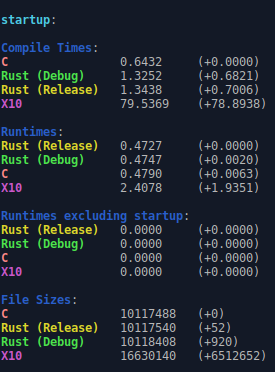
\includegraphics[height=200px]{eval-screenshots/startup.png}  
\end{center}

Anhand dieser Werte kann man prinzipiell erkennen, dass die Anlaufzeiten von C und Rust sich sehr nahe sind, während X10
hierfür ca. 2 Sekunden länger benötigt. Außerdem benötigt das X10 Programm weitaus länger um die Kompilierung auszuführen und
weist eine deutlich größere Dateigröße auf.

\subsection{Berechnen von Primzahlen}

Um die Rechenleistung der verschiedenen Programmiersprachen bei einem intensiveren Problem zu vergleichen, wurden
Programme geschrieben welche Primzahlen berechnen. Hierbei wurden zwei unterschiedliche Ansätze verwendet: Zum einen
eine naive Berechnung, welche jede Zahl individuell auf Teilbarkeit mit kleineren Zahlen prüft und andererseits
das Sieb von Eratosthenes, eine effiziente Methode zum Berechnen von Primzahlen.

\begin{center}
	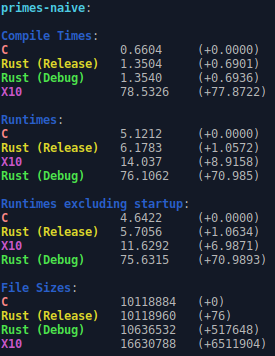
\includegraphics[height=200px]{eval-screenshots/primes-naive.png}
	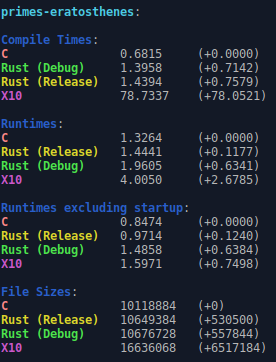
\includegraphics[height=200px]{eval-screenshots/primes-eratosthenes.png}
\end{center}

Hier erkennt man bereits einige Leistungsunterschiede zwischen den Programmiersprachen. Während C die unangefochten
beste Laufzeit aufweist, hinkt Rust nicht signifikant hinterher, während die Lauzeit des X10-Programms auch nach Abzug
der größeren Anlaufzeit schlechter als die beiden Systemsprachen abschneidet.


\subsection{Müll-Ersteller}

X10 verwaltet den Speicher mithilfe eines Garbage Collectors, wobei C und Rust ohne einen solchen auskommen.
Während Garbage Collector ein sehr hilfreiches Werkzeug sind, um den Programmieraufwand zu verringern, so kommt dies
allerdings auch auf Kosten der Laufzeiteffizienz, vor allem die Garbage-Collector-Pause ist hier ein nicht zu unterschätzender
Faktor.

Um diese Leistungsdifferenz zu veranschaulichen, wurde ein Benchmark-Programm geschrieben, welche kontinuierlich
Objekte auf dem Heap erstellt, welche anschließend wieder aus dem gültigen Anwendungsbereich verschwindet.

\begin{center}
	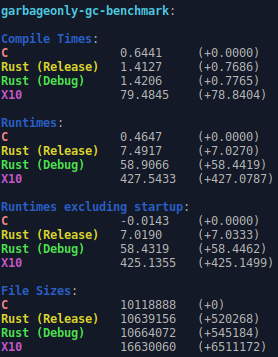
\includegraphics[height=300px]{eval-screenshots/garbageonly.png}
\end{center}

Wie man an den Ergebnissen des Benchmarks erkennen kann, benötigt X10 deutlich länger um die selbe Anzahl und gleich große
Objekte zu erstellen als C oder Rust. Dies weist darauf hin dass der Garbage Collector unter Umständen einen signifikanten
Einfluss auf das Laufzeitverhalten haben kann. C und Rust haben hier also einen Vorteil, vor allem Rust, denn
diese Sprache bietet eine ähnliche Speichersicherheit wie es Sprachen mit Garbage Collector bieten.


\section{Sicherheit}

Im folgenden wird die Sicherheit bezüglich undefiniertem Verhalten als Folge von fehlerhaften Speicherzugriffen analysiert.
Hierbei ist vor allem der Vergleich zwischen Rust und C interessant, da einige von Rusts primären Eigenschaften die
Risiken der C-Programmierung beseitigen sollen.

\subsection{Division durch 0}

Dividiert man in C einen Wert durch die Zahl 0, kann es zu undefiniertem Verhalten führen, welches generell
unerwünschtes Verhalten darstellt. Versucht man dies in Rust, so stürzt das Programm sofort ab, es kann nicht zu undefiniertem
Verhalten kommen.

\subsection{Pufferüberlauf}

Ein weiterer Fall, der in C zu undefiniertem Verhalten führt, sind Pufferüberläufe. Diese geschehen, wenn man beispielsweise
in einem Array der Größe n versucht, auf das n+1te Element zuzugreifen. Wie bereits im letzten Vergleich kann dies in 
Rust nicht geschehen, da das Programm abstürzt.

\subsection{Nicht Initialisierte Variablen}

In C ist es möglich, uninitialiserte Variablen zu verwenden, dies führt allerdings zu undefiniertem Verhalten. In Rust hingegen
wird dies bereits vom Compiler verhindert, da er den Gebrauch von uninitialisierten Variablen verbietet. Ein Rust-Programm
welches also uninitialisierte Variablen verwendet kompiliert also gar nicht und kann so natürlich auch nicht
zu undefiniertem Verhalten führen.


\section{Abstraktionen}

Es werden nun die implementierten Abstraktionen der octolib Bibliothek mit den Implementierungen in C und X10 verglichen.

\subsection{Minimales Infect}

\subsection{Cleanup}

\subsection{Closures}

Closures bieten eine praktische Art und Weise, anonyme Funktionen zu nutzen



\chapter{Fazit und Ausblick}\label{sec:conclusion}

Im Folgenden werden die Ergebnisse der Evaluation bewertet
und ein Ausblick auf die Zukunft der Programmiersprache Rust im Bezug zum invasiven Rechnen geboten.

\section{Fazit}

Betrachtet man die Ergebnisse der Evaluation, so kann behauptet werden,
dass Rust in gewissen Aspekten C oder X10 vorzuziehen ist.

Zum einen eliminiert Rust einige Fehlerquellen, welche in C oder anderen herkömmlichen
Systemsprachen zu undefiniertem Verhalten führen können.
In Rust muss der Programmierer nicht selbst auf solche Fehler achten und wird bereits vom Compiler auf Fehler
hingewiesen. Dies erlaubt es, sicherere und weniger fehleranfällige Programme zu schreiben.
Sollte es trotzdem während der Laufzeit zu schwerwiegenden Fehlern kommen, beispielsweise bei einem Pufferüberlauf,
brechen Rust Programme die Ausführung ab und weisen so kein undefiniertes Verhalten auf.

Des Weiteren weist Rust in Situationen, in denen häufig Objekte erstellt und wieder den Geltungsbereich verlassen,
ein mindestens 10-fach besseres Laufzeitverhalten auf als X10.
Zudem eignet sich X10 wegen des \textit{Garbage Collectors}
nicht für Anwendungsgebiete, in denen Pausen jeglicher Art nicht erwünscht sind,
beispielsweise bei Echtzeitsystemen.
In diesem Einsatzgebiet ist die Verfügbarkeit des Systems wichtig, daher wäre eine \textit{Garbage Collector}-Pause
nicht wünschenswert. Rust wäre hier eine bessere Option.

Außerdem weist das Kompilieren mit \textit{octorust} eine 100- bis 200-fach kürzere Kompilierungsdauer
als der \textit{x10i}-Compiler auf. Dies kann bei der Entwicklung von Programmen ein Zeitersparnis von
mehreren Minuten pro Kompilierungsvorgang zur Folge haben. 
Zudem sind die Dateigrößen der kompilierten Rust Programme im betrachteten Minimalfall 6511716 Byte kleiner
als die Größe eines kompilierten invasiven X10 Programms.

Rust bietet beim Programmieraufwand kaum Vorteile gegenüber X10, einzig das implizite \textit{Retreat} wäre hier zu 
erwähnen.
X10 bietet zudem derzeit robustere Abstraktionen über die C-Schnittstelle von \textit{OctoPOS} und
\textit{iRTSS}.
Vergleicht man Rust diesbezüglich allerdings mit C, so erkennt man eine deutliche Reduktion im Programmieraufwand.

Negativ zu betrachten wäre die starke Abhängigkeit von der \textit{OctoPOS/iRTSS} C-Schnittstelle,
welche die Sicherheit von Rust teils aufgibt. Die Funktionen der C-Schnittstelle bieten nämlich keine Garantien 
bezüglich der Sicherheit und die häufige Nutzung von \texttt{\textsc{\textbf{void}}}-Zeigern zum Übertragen
von Parametern ist ebenfalls ein Problem, welches zu Fehlern führen kann.

\section{Ausblick}

Da Rust noch eine relativ junge Programmiersprache ist, wurden viele Bibliotheken für diese noch nicht implementiert.
Zwar können mithilfe der \textit{Foreign Function Interface} Bibliotheken,
die in anderen Sprachen geschrieben worden sind, eingebunden werden, diese bieten jedoch
nicht die Sicherheitsgarantien wie Rust es tut.
In dieser Hinsicht sollte sich die Lage jedoch in der Zukunft verbessern, wenn Rust
weiterhin gerne von Entwicklern genutzt wird und eventuell großflächiger zum Einsatz kommt.

Eine weitere Möglichkeit in der Zukunft ist die Portierung der Standardbibliothek auf die SPARC-V8 Architektur.
Die Standardbibliothek bietet einige hilfreiche Konstrukte und Funktionen,
die das Programmieren erleichtern und sicherer machen.
Möglich wäre es, dass die Entwickler der Rust Programmiersprache selbst die SPARC-V8 Architektur
in der Zukunft unterstützen und so die Standardbibliothek portiert wird. Alternativ wäre es möglich, dass die 
Standardbibliothek im Rahmen des invasiven Rechnen portiert wird, sollte genügend Interesse daran bestehen.

Durch die unsichere Art und Weise, in der die Parameterübergabe in der \textit{Infect}-Phase derzeit in
\textit{octolib} angeboten wird, können Programmfehler entstehen. Dies könnte beispielsweise durch den Einsatz von
Serialisierungsbibliotheken wie \texttt{\textsc{\textbf{serde}}} in der Zukunft verbessert werden.

Um die starke Abhängigkeit von der \textit{OctoPOS/iRTSS} C-Schnittstelle zu verringern,
können weitere Abstraktionen erstellt werden, welche von den
besonderen Eigenschaften der Rust-Programmiersprache Gebrauch machen.
Dass dies möglich ist, hat die Implementierung des X10-Compilers \textit{x10i} bewiesen,
denn dieser verwendet dieselbe C-Schnittstelle,
bietet jedoch robuste Abstraktionen über diese und erlaubt so
das Entwickeln von X10-Programmen, ohne dass der Programmierer sich dabei mit der C-Schnittstelle befassen muss.


\bibliographystyle{ieeetr}
\bibliography{bib}

\begin{otherlanguage}{ngerman}
\chapter*{Erklärung}
\pagestyle{empty}

  \vspace{20mm}
  Hiermit erkläre ich, \theauthor, dass ich die vorliegende Bachelorarbeit selbst\-ständig
verfasst habe und keine anderen als die angegebenen Quellen und Hilfsmittel
benutzt habe, die wörtlich oder inhaltlich übernommenen Stellen als solche kenntlich gemacht und
die Satzung des KIT zur Sicherung guter wissenschaftlicher Praxis beachtet habe.
  \vspace{20mm}
  \begin{tabbing}
  \rule{4cm}{.4pt}\hspace{1cm} \= \rule{7cm}{.4pt} \\
 Ort, Datum \> Unterschrift
  \end{tabbing}
\end{otherlanguage}

\chapter*{Danksagung}
\pagestyle{empty}

Ich danke meinen Eltern Janine und Heinz als auch meinem Bruder Michael, die mich meine gesamtes Leben lang durch dick und dünn
begleitet und unterstützt haben. Außerdem danke ich meinen guten Freunden Simon Eherler und Frederick Horn, ohne die ich nicht der
Mensch wäre der ich heute bin. Ich danke meinen Kommilitonen Marius Take, Johannes Bucher, Thomas Schmidt und Daniel Mockenhaupt,
ohne die mein Studium am KIT nicht halb so schön wäre. Ich danke meiner "`Ersatzfamilie"', der Familie Eherler,
die immer einen Platz in ihrer Mitte für mich hat. Ich danke meinem Betreuer Andreas Zwinkau, welcher
mich freundlich und hilfreich durch die Erstellung dieser Arbeit begleitet hat. Und zu guter Letzt
danke ich dem Karlsruher Institut für Technologie, welches es mir erst ermöglichte, dieses Studium zu absolvieren.

\pagestyle{fancy}
\appendix

%\chapter{Sonstiges}

\section{Anmeldung}

Üblicherweise melden wir eine Arbeit erst an,
wenn der Student mit dem Schreiben begonnen hat,
also nach der Implementierung.
Das verringert die Bürokratie und den Stress,
der mit verpassten Deadlines kommt.

Außerdem ist ein Abbrechen nach der Anmeldung ein offizieller Akt
für den es wiederum Fristen gibt:

\begin{center}
\begin{tabular}{lrrr}
\toprule
 & Abbruchfrist nach Anmeldung \\
\midrule
Bachelor      & 4 Wochen \\
Master        & 2 Monate \\
Diplom        & 3 Monate \\
\bottomrule
\end{tabular}
\end{center}

Nach dieser Frist muss die abgebrochene Arbeit mit 5,0 bewertet werden.

Das ISS empfiehlt, dass Studenten sich zusätzlich selbst im Studienportal anmelden.
Das könnte die Eintragung der Note beschleunigen.

\section{Antrittsvortrag}

Bei internen Arbeiten jeglicher Art ist ein Antrittsvortrag optional.
Bei externen Arbeiten ist ein Antrittsvortrag Pflicht.

Dauer: 15 Minuten + 5 Minuten Fragezeit.

Ein Antrittsvortrag sollte nach der Einarbeitungsphase stattfinden,
wenn man einen Überblick hat und weiß was man vorhat.
Im Antrittsvortrag kann man abtasten was Prof.~Snelting von dem Thema hält
und wo man Schwerpunkte setzen oder erweitern sollte.

\section{Abgabe}

\begin{center}
\begin{tabular}{lrrr}
\toprule
 & Dauer & Umfang \\
\midrule
Bachelor      & 4 Monate & 30+ Seiten \\
Master        & 6 Monate & 50+ Seiten \\
Studienarbeit & 3 Monate & 30+ Seiten \\
Diplom        & 6 Monate & 50+ Seiten \\
\bottomrule
\end{tabular}
\end{center}

Man kann eine "4.0 Bescheinigung" bekommen,
bspw.\ für die Masteranmeldungen.

Abzugeben sind jeweils 4 gedruckte Examplare der Arbeit,
das Dokument als pdf Datei
und entstandener Code und andere Artefakte.
Außerdem könnten spätere Studenten dankbar sein für \TeX-Sourcen.

Zum Drucken empfehlen wir
Katz Copy\footnote{\url{http://www.katz-copy.com/}} am Kronenplatz,
weil wir in Sachen Qualität dort die besten Erfahrungen gemacht haben.
Bitte keine Spiralbindung,
da sich das schlecht Stapeln lässt.
Farbdruck ist nicht verpflichtend,
solange in Schwarzweiß noch alle Grafiken lesbar sind.

\section{Abschlussvortrag}

Die Abschlusspräsentation dauert für Bachelorarbeiten 15 Minuten
zuzüglich mind. 10 Minuten für Fragen.
Bei Masterarbeiten sind 20--25 Minuten für den Vortrag vorgesehen.

Der Vortrag soll innerhalb von vier Wochen nach Abgabe erfolgen,
entsprechend Prüfungsordnung.
Die Arbeit muss mindestens einen Tag vor dem Abschlussvortrag abgegeben sein,
damit sich Prof.~Snelting vorbereiten kann.

Am besten direkt im Anschluß den Vortrag ausarbeiten und ein oder zwei Wochen nach Abgabe halten.
Der Präsentationstermin muss ein bis zwei Monate im Voraus geplant werden,
denn Prof.~Snelting hat üblicherweise einen vollen Terminkalender.

\section{Gutachten}

Der Prüfer erstellt ein Gutachten zur Arbeit.
Um das Gutachten einzusehen muss ein Antrag beim Prüfungsamt gestellt werden.
Der Betreuer bzw. Prüfer darf das Gutachten nur mit genehmigtem Gutachten zeigen.
Mündliche Auskunft zur Note ist allerdings möglich.

\section{Bewertung}

\begin{itemize}
  \item Diplom- und Masterarbeiten \emph{müssen} eine wissenschaftliche Komponente enthalten.
    Bachelorarbeit \emph{sollten}, aber zum Bestehen ist es nicht notwendig.
    Wissenschaftlich ist was über reine Implementierungs- bzw. Softwareentwicklungsaufgaben hinausgeht.
    Üblicherweise findet man theoretische Betrachtungen zu Korrektheit und Effizienz.
    Willkürliche Daumenregel: Ohne Formel, keine Wissenschaft.
  \item Diplom- und Masterarbeiten benötigen eigentlich immer Wissen aus dem Diplom- bzw. Masterstudium.
    Falls das Wissen aus Vordiplom bzw. Bachelor ausreicht,
    sollte man nochmal darüber nachdenken.
  \item Positiv mit der Note korrelieren
    selbstständiges Arbeiten,
    regelmäßige Abstimmung mit dem Betreuer,
    mehrere Feedbackrunden mit verschiedenen Leuten,
    mehrmaliges Üben des Abschlussvortrags,
    Einbringen eigener Ideen,
    gutes Zuhören
    und sorgfältiges Debugging.
  \item Negativ mit der Note korrelieren
    wochenlanges Pausieren,
    Ignorieren von Feedback,
    Deadlines überziehen
    und Arbeiten im stillen Kämmerchen.
\end{itemize}

Disclaimer:
Nein, es gibt keinen konkreten Notenschlüssel.
Die obigen Punkte sind nur grobe Richtlinien und für niemanden in irgendeiner Weise bindend.

\section{\LaTeX\ Features}

\subsection{Schriftformatierungen}

\begin{tabular}{lccc}
\toprule
 & serif & sans-serif & fixed-width \\
\midrule
normal        & \textrm{\textup{Medium}} \textrm{\textup{\textbf{Bold}}} & \textsf{\textup{Medium}} \textsf{\textup{\textbf{Bold}}} & \texttt{\textup{Medium}} \texttt{\textup{\textbf{Bold}}} \\
italic        & \textrm{\textit{Medium}} \textrm{\textit{\textbf{Bold}}} & \textsf{\textit{Medium}} \textsf{\textit{\textbf{Bold}}} & \texttt{\textit{Medium}} \texttt{\textit{\textbf{Bold}}}\\
slanted       & \textrm{\textsl{Medium}} \textrm{\textsl{Bold}} & \textsf{\textsl{Medium}} \textsf{\textsl{\textbf{Bold}}} & \texttt{\textsl{Medium}} \texttt{\textsl{\textbf{Bold}}} \\
small-capital & \textrm{\textsc{Medium}} \textrm{\textsc{\textbf{Bold}}} & \textsf{\textsc{Medium}} \textsf{\textsc{\textbf{Bold}}} & \texttt{\textsc{Medium}} \texttt{\textsc{\textbf{Bold}}} \\
\bottomrule
\end{tabular}

Math fonts:
$\mathnormal{absXYZ}$,
$\mathrm{absXYZ}$,
$\mathbf{absXYZ}$,
$\mathsf{absXYZ}$,
$\mathit{absXYZ}$,
$\mathtt{absXYZ}$, and
$\mathcal{XYZ}$.

\subsection{Rand und Platz}

Viele Benutzer von \LaTeX\ wollen Ränder und Seitengröße anpassen.
Dazu empfehlen wir erstmal die KOMA Script Dokumentation (\texttt{koma-script.pdf}) zu lesen,
insbesondere Kapitel 2.2.
Bevor man mit \texttt{\textbackslash enlargethispage}
oder ähnlichen Tricks anfängt,
sollte man \texttt{\textbackslash typearea} anpassen.

Falls die Arbeit auf Englisch verfasst wird,
sollte man wissen, dass Absätze im Englischen üblicherweise anders formatiert werden.
Im Deutschen macht man eine Leerzeile zwischen Absätzen.
Im Englischen wird stattdessen die erste Zeile eines Absatzes eingerückt.


\end{document}
